\documentclass[a4]{beamer}
\usepackage{amssymb}
\usepackage{graphicx}
\usepackage{subfigure}
\usepackage{newlfont}
\usepackage{amsmath,amsthm,amsfonts}
%\usepackage{beamerthemesplit}
\usepackage{pgf,pgfarrows,pgfnodes,pgfautomata,pgfheaps,pgfshade}
\usepackage{mathptmx} % Font Family
\usepackage{helvet} % Font Family
\usepackage{color}
\mode<presentation> {
\usetheme{Default} % was Frankfurt
\useinnertheme{rounded}
\useoutertheme{infolines}
\usefonttheme{serif}
%\usecolortheme{wolverine}
% \usecolortheme{rose}
\usefonttheme{structurebold}
}
\setbeamercovered{dynamic}
\title[MA4413]{Statistics for Computing \\ {\normalsize MA4413 Lecture 11A}}
\author[Kevin O'Brien]{Kevin O'Brien \\ {\scriptsize kevin.obrien@ul.ie}}
\date{Autumn 2013}
\institute[Maths \& Stats]{Dept. of Mathematics \& Statistics, \\ University \textit{of} Limerick}
\renewcommand{\arraystretch}{1.5}
%------------------------------------------------------------------------%

\begin{document}
\begin{frame}
\titlepage
\end{frame}

\begin{frame}
\frametitle{Discrete memoryless channel (from last lecture)}
\begin{itemize}
\item For a DMC with ``m" inputs and ``n" outputs, the input X consists of input symbols $x_1, x_2, \ldots x_m$.
\item The probabilities of these source symbols $P(x_i)$ are assumed to be known.
\item The output Y consists of output symbols $\{y_1,y_2,\ldots, y_n \}$
\item Each possible input-to-output path is indicated along with a conditional probability $P(y_j|x_i)$, where $P(y_j|x_i)$  is the conditional probability of
obtaining output $y_j$ given that the input is $x_i$. \item $P(y_j|x_i)$ is called a \textbf{\emph{channel transition probability}}.
\end{itemize}
\end{frame}
%\end{document}
%--------------------------------------------------------%
%--------------------------------------------------------%
\begin{frame}
\frametitle{Discrete memoryless channel}
\vspace{-1cm}
\begin{itemize}
\item On the next slide, we present a binary DMC, with the channel transition probabilities indicated.
\item $P(y_1|x_1)$ = 0.9  and $P(y_2|x_1)$ = 0.1
\item $P(y_1|x_2)$ = 0.2  and $P(y_2|x_2)$ = 0.8
\end{itemize}
\end{frame}

\begin{frame}
\frametitle{Discrete Memoryless Channels}

\begin{center}
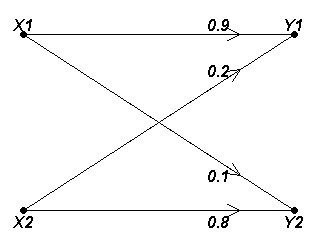
\includegraphics[scale=0.54]{images/10Bnet2}
\end{center}
\end{frame}
%---------------------------------------------------------------------------------------------------------------------------------------------------%
\begin{frame}
\frametitle{Types of Channel}
\textbf{ 1. Lossless Channel:}\\
A channel described by a channel matrix with only one non-zero element in each column is called a lossless channel.


\[  [P(Y|X)]  =  \left[ \begin{array}{ccccc}
3/4 & 1/4 &0 & 0&0\\
0  & 0 &1/3 & 2/3& 0\\
0  & 0& 0&0 &1 \\
\end{array} \right]  \]
%(Drawn in overhead):\\ \bigskip

It can be shown that in the lossless channel, no source information is lost in transmission.
\end{frame}
%---------------------------------------------------------------------------------------------------------------------------------------------------%
\begin{frame}
\frametitle{Types of Channel}
\textbf{ 1. Lossless Channel:}\\

\begin{figure}
\centering
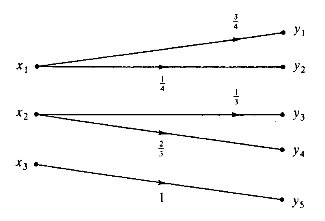
\includegraphics[width=0.7\linewidth]{images/11Blossless}
\caption{}
\label{fig:11Blossless}
\end{figure}


\end{frame}

%---------------------------------------------------------------------------------------------------------------------------------------------------%
\begin{frame}
\frametitle{Types of Channel}
\textbf{2. Deterministic Channel:}\\
A channel described by a channel matrix with only one non-zero element in each row is called a deterministic channel.

\[  [P(Y|X)]  =  \left[ \begin{array}{ccc}
1   & 0 &0 \\
1  & 0 &0\\
0  & 1 &0\\
0  & 1& 0 \\
0  & 0& 1 \\
\end{array} \right]  \]
%(Drawn in overhead):\\ \bigskip
Note that since each row has only one non-zero element, this element must be 1. When a given source symbol is sent in a deterministic channel, it is clear which output symbol would be received.
\end{frame}

%---------------------------------------------------------------------------------------------------------------------------------------------------%
\begin{frame}
\frametitle{Types of Channel}
\textbf{2. Deterministic Channel:}\\
\begin{figure}
\centering
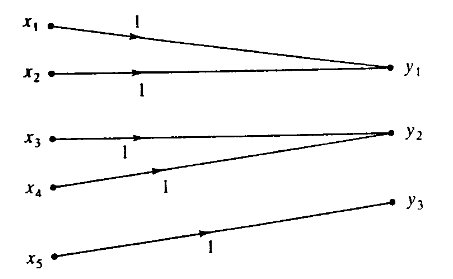
\includegraphics[width=0.7\linewidth]{images/11Bdeterministic}
\caption{}
\label{fig:11Bdeterministic}
\end{figure}

\end{frame}

%---------------------------------------------------------------------------------------------------------------------------------------------------%
\begin{frame}
\frametitle{Types of Channel}
\textbf{3. Noiseless Channel:}\\
A channel is said to be \emph{\textbf{noiseless}} if it is both lossless and deterministic.
The channel matrix is the identity matrix: only one element in each row and each column, and each element is necessarily 1.
\[  [P(Y|X)]  = \left[ \begin{array}{cccc}
1 &0 & \ldots & 0 \\
0 & 1& \ldots & 0 \\
\ldots & \ldots & \ldots & \ldots \\
0& 0 & \ldots & 1 \\
\end{array} \right] \]
%(Drawn in overhead):\\ \bigskip
Note that the input and output alphabets have the same size , i.e. $m=n$.
\end{frame}
\begin{frame}
\frametitle{Types of Channel}
\textbf{3. Noiseless Channel:}\\
\begin{figure}
\centering
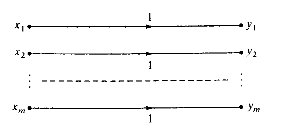
\includegraphics[width=0.7\linewidth]{images/11BNoiseless}
\caption{}
\label{fig:11BNoiseless}
\end{figure}

\end{frame}
%----------------------------------------------------------------------------------------------------------------------------------------------------%
\begin{frame}
\frametitle{Types of Channel}
\textbf{4. Binary Symmetric Channel:}\\
The binary symmetric channel is defined by the following channel diagram (next slide) and the channel matrix is given by

\[  [P(Y|X)]  = \left[ \begin{array}{cc}
1-p & p  \\
p & 1-p\\
\end{array} \right] \]
The channel has two inputs and two outputs $(x_1=0,x_2=1)$ and two outputs $(x_1=0,x_2=1)$. The channel is symmetric because the probability of receiving a 1 if a 0 is sent is the same as the probability of receiving a 0 if a 1 was sent. This common probability is denoted $p$.
\end{frame}

\frame{
\frametitle{Binary Symmetric Channels}

\begin{center}
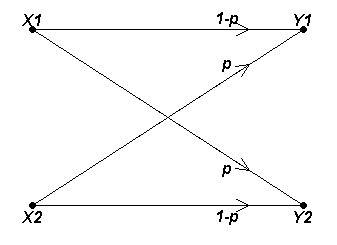
\includegraphics[scale=0.54]{images/11aBSC}
\end{center}
}



\end{document}
%---------------------------------------------------------------------------------------------------------------------------------------%


\end{document}


%----------------------------------------------------------------Part 4 Huffman Coding-%

\frame{
\frametitle{Huffman encoding algorithm}
Huffman coding is an entropy encoding algorithm used for lossless data compression.\\
\bigskip
A frequency based coding scheme (algorithm) that follows Huffman's idea is called Huffman coding. Huffman coding is a simple algorithm that generates a set of variable-size codewords of the minimum average length. The algorithm for Huffman encoding involves the following steps:
}
%--------------------------------------------------------------Part 4 Huffman Coding-%

\frame{
\begin{itemize}
\item[1.] Frequency Table: Constructing a frequency table sorted in descending order.

\item[2.] Building a binary tree:
    Carrying out iterations until completion of a complete binary tree:
    \begin{itemize}
    \item[(a)] Merge the last two items (which have the minimum frequencies) of    the frequency table to form a new combined item with a sum
    frequency of the two.
    \item[(b)] Insert the combined item and update the frequency table.
    \end{itemize}

\item[3.] Deriving Huffman tree:
Starting at the root, trace down to every leaf; mark �0� for a left branch and �1� for a right branch.

\item[4.] Generating Huffman code:
Collecting the 0s and 1s for each path from the root to a leaf and assigning a 0-1 codeword for each symbol.

\end{itemize}
}
%--------------------------------------------------------------------------Part 4 Huffman Coding-%

\frame{

Huffman coding is a method of lossless data compression, and a form of entropy encoding. The basic idea is to map an alphabet to a representation for that alphabet, composed of strings of variable size, so that symbols that have a higher probability of occurring have a smaller representation than those that occur less often.

}
%-------------------------------------------------------------------------------Part 4 Huffman Coding-%

\frame{
The key to Huffman coding is Huffman's algorithm, which constructs an extended binary tree of minimum weighted path length from a list of weights. For this problem, our list of weights consists of the probabilities of symbol occurrence. From this tree (which we will call a Huffman tree for convenience), the mapping to our variable-sized representations can be defined.
}
%-----------------------------------------------------------------------Part 4 Huffman Coding-%
\frame{
The mapping is obtained by the path from the root of the Huffman tree to the leaf associated with a symbol's weight. The method can be arbitrary, but typically a value of 0 is associated with an edge to any left child and a value of 1 with an edge to any right child (or vice-versa). By concatenating the labels associated with the edges that make up the path from the root to a leaf, we get a binary string. Thus the mapping is defined.
}
%-------------------------------------------------------------------------------------------%
\frame{
\frametitle{Inverse Mapping}
\begin{itemize}
\item In order to recover the symbols that make up a string from its representation after encoding, an inverse mapping must be possible. It is important that this mapping is unambiguous. \item We can show that all possible strings formed by concatenating any number of path labels in a Huffman tree are indeed unambiguous, due to the fact that it is a complete binary tree. \item That is, given a string composed of Huffman codes, there is exactly one possible way to decompose it into the individual codes.
\end{itemize}
}

\frame{
\frametitle{Data compression(2)}
The key approaches of data compression can be summarized as modelling + coding.
Modelling is a process of constructing a knowledge system for
performing compression. Coding includes the design of the code and product of the compact data form.

}

% - Entropy
% - Information
% - Mutual Information



%-------------------------------------------------------------------------------------------------------------------------------------------------------------------------------------------%


% page 247






%r. - · yi
%XI: X Ptytnt ykzyr
%rn,. · yn



\begin{frame}
\frametitle{Code efficiency and Code redundancy}
% Pg 253/254
The parameter $L$ represents the average number of bits per source symbol used in the source coding process.
The code efficiency is defined as \[\nu = {L_{min} \over L} \]where $L_{min}$ is the minimum possiblve value of $L$. When $\nu$ approaches unity, the codes is said to be efficient.
The code redundancy $\gamma$ is defined as $\gamma = 1- \nu$.
\end{frame}


%---------------------------------------------------------------------------------------------------------------------------------------%
\begin{frame}
%page 254
\frametitle{Source Coding Theorem}
The source coding theorem states that for zi DMS X with entropy $H(X)$, the average code word length $L$ per symbol is bounded as
L 2 H(X) (10.52)

and further, L can bc made as close to H(X) as dcsircd for some suitably chosen code.
Thus, with$ L_{min} \geq H(X)$.

The code efficiency can be rewritten as
\[\nu = {H(X) \over L} \]
\end{frame}

%-----------------------------------------------------------------------------------------------------------------------------------------------------------%
\begin{frame}
\frametitle{ Kraft inequality}
\begin{itemize}
\item Let X be a DMS with alphabet ($x _i = \{1, 2, . . . ,m\}$). Assume that the length of the assigned binary
code word corresponding to x, is n,.
\item A necessary and sufficient condition for the existence of an instantaneous binary code is

 \[ K = \sum^{m}_{i=1}2^{-n_i} \leq 1 \]
which is known as the \textbf{Kraft inequality}.
\item Note that the Kraft inequality assures us of the existence of an instantaneously decodable code
with code word lengths that satisfy the inequality. But it does not show us how to obtain these code
words, nor does it say that any code that satisfies the inequality is automatically uniquely decodable
\end{itemize}
\end{frame}

\end{document}
















%-----------------------------------------------------------------------------------------------%
\begin{frame} % ULCIS
\frametitle{Self Information}Self-information
This is defined by the following mathematical formula:$I(A) = −logb P(A)$

The self-information of an event measures the amount of one's surprise
evoked by the event. The negative logarithm $−logb P(A)$ can also be written as \[
log_b  {1 \over P(A)} \]
Note that log(1) = 0, and that $| − log(P(A))|$ increases as P(A) decreases
from 1 to 0. This supports our intuition from daily experience. For example,
a low-probability event tends to cause more ``surprise".
\end{frame}


%-------------------------------------------------------------------------------------------%
\frame{
\frametitle{Example}
For a simple example, we will take a short phrase and derive our probabilities from a frequency count of letters within that phrase. The resulting encoding should be good for compressing this phrase, but of course will be inappropriate for other phrases with a different letter distribution.

"All you base are belong to us"
}


%----------------------------------------------------------------------------------%
\frame{
\frametitle{Entropy}
\begin{itemize}
\item Entropy is the uncertainty of a single random variable. \item We can define \textbf{\emph{conditional entropy }}$H(X|Y)$, which is the entropy of a random variable
conditional on the knowledge of another random variable. \item The reduction in uncertainty due to another random variable is called the \textbf{\emph{mutual information}}.
\end{itemize}
}
%----------------------------------------------------------------------------------%



\frame{
\frametitle{What is Information?}
\begin{itemize} \item Once we agree to define the information of an event ain terms of P(a), the properties (2) and (3) will be satisfied if the information in ais defined as
\[ I(a) = -log P(a)\]

\item Remark : The base of the logarithm depends on the unit of information to be used.
\end{itemize}
}



%-------------------------------------------------------------------------------------------%
\frame{
Ambiguity occurs if there is any path to some symbol whose label is a prefix of the label of a path to some other symbol. In the Huffman tree, every symbol is a \textbf{\emph{leaf}}. Thus it is impossible for the label of a path to a leaf to be a prefix of any other path label, and so the mapping defined by Huffman coding has an inverse and decoding is possible.
}
%-------------------------------------------------------------------------------------------%
\frame{
\frametitle{Example}
For a simple example, we will take a short phrase and derive our probabilities from a frequency count of letters within that phrase. The resulting encoding should be good for compressing this phrase, but of course will be inappropriate for other phrases with a different letter distribution.

"All you base are belong to us"
}




\end{document}